\documentclass[11pt]{article}

\usepackage{fullpage}
\usepackage{amsfonts}
\usepackage{amssymb}
\usepackage{mdwlist}
\usepackage[usenames,dvipsnames]{xcolor}
\usepackage{tikz}

\newcommand{\coursenum}{CS172}
\newcommand{\coursename}{Automata, Computability and Complexity}
\newcommand{\courseprof}{Professor Luca Trevisan}

%       Usage: \ptitle{title}{dateout}
\newcommand{\ptitle}[2]{\noindent\parbox{\textwidth}
{U.C. Berkeley --- \coursenum : \coursename \hfill #1 \newline
\courseprof \hfill #2 \newline
\mbox{}\hrulefill\mbox{}}\vspace*{1ex}\mbox{}\newline
\bigskip
\begin{center}{\Large\bf #1}\end{center}
\bigskip}


%       Usage: \handout{title}{datelec}{dateout}{scribe}
\newcommand{\handout}[2]{\thispagestyle{empty}
 \markboth{Notes for Lecture #1}{Notes for Lecture #1}
 \pagestyle{myheadings}\htitle{#1}{#2}}

%       Usage: \pset{title}{dateout}
\newcommand{\pset}[2]{\thispagestyle{empty}
 \markboth{#1 --- #2}{#1 --- #2}
 \pagestyle{myheadings}\ptitle{#1}{#2}}





\begin{document}

\ptitle{Problem Set 2}{January 29, 2015}

This problem set is due on Friday, February 6, by 5pm. Please submit your solution online using bcourses,
as a pdf file. 

You can type your solution, or handwrite it. If you handwrite it, then either
scan it or take a good resolution picture of each page and then collate the pictures
and export them to a {\em single} pdf file.

\bigskip

\hrule

\section*{Problem 1: DFA to Regex (20/100)}

Convert the following DFA to a regular expression.\\

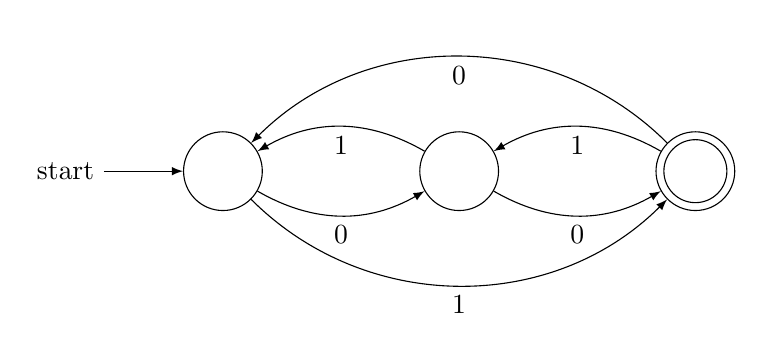
\begin{tikzpicture}
  \node (label) at (-2, 0) {start};
  \node[draw,circle,minimum size=1cm] (node0) at (0,0) {};
  \node[draw,circle,minimum size=1cm] (node1) at (3,0) {};
  \node[draw,circle,minimum size=1cm] (node2) at (6,0) {};
  \node[draw,circle,minimum size=0.8cm] (node3) at (6,0) {};
  \path [-latex] (label) edge (node0);
  \path [-latex] (node0) edge [bend right] node[below] {0} (node1);
  \path [-latex] (node1) edge [bend right] node[below] {0} (node2);
  \path [-latex] (node0) edge [bend right=45] node[below] {1} (node2);
  \path [-latex] (node2) edge [bend right] node[below] {1} (node1);
  \path [-latex] (node1) edge [bend right] node[below] {1} (node0);
  \path [-latex] (node2) edge [bend right=45] node[below] {0} (node0);
\end{tikzpicture}

\section*{Problem 2: DFA to Regex (20/100)}

Convert the following DFA to a regular expression.\\

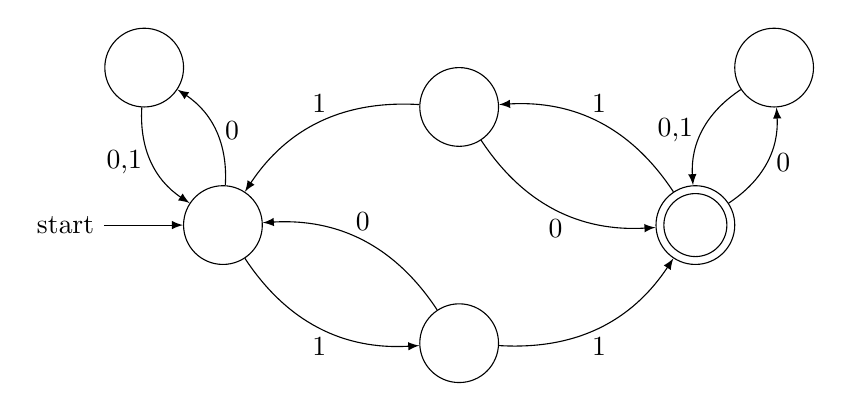
\begin{tikzpicture}
  \node (label) at (-2, 0) {start};
  \node[draw,circle,minimum size=1cm] (node0) at (0,0) {};
  \node[draw,circle,minimum size=1cm] (node0waste) at (-1,2) {};
  \node[draw,circle,minimum size=1cm] (node1waste) at (7,2) {};

  \path [-latex] (node0) edge [bend right] node[right] {0} (node0waste);
  \path [-latex] (node0waste) edge [bend right] node[left] {0,1} (node0);

  \node[draw,circle,minimum size=1cm] (node0to1) at (3,-1.5) {};

  \node[draw,circle,minimum size=1cm] (node1to0) at (3, 1.5) {};

  \node[draw,circle,minimum size=0.8cm]  at (6,0) {};
  \node[draw,circle,minimum size=1cm] (node1) at (6,0) {};

  \path [-latex] (label) edge (node0);
  
  \path [-latex] (node1) edge [bend right] node[right] {0} (node1waste);
  \path [-latex] (node1waste) edge [bend right] node[left] {0,1} (node1);

  
  \path [-latex] (node0) edge [bend right] node[below] {1} (node0to1);
  \path [-latex] (node0to1) edge [bend right] node[above] {0} (node0);


  \path [-latex] (node0to1) edge [bend right] node[below] {1} (node1);


  \path [-latex] (node1) edge [bend right] node[above] {1} (node1to0);
  \path [-latex] (node1to0) edge [bend right] node[below] {0} (node1);

  \path [-latex] (node1to0) edge [bend right] node[above] {1} (node0);

  
\end{tikzpicture}


\section*{Problem 3: NFA to Regex (20/100)}

Convert the following DFA to a regular expression.\\

\begin{tikzpicture}
  \node (label) at (-2, 0) {start};
  \node[draw,circle,minimum size=1cm] (node0) at (0,0) {};
  \node[draw,circle,minimum size=1cm] (node1) at (3,0) {};
  \node[draw,circle,minimum size=1cm] (node2) at (6,0) {};
  \node[draw,circle,minimum size=1cm] (node3) at (6,3) {};
  \node[draw,circle,minimum size=1cm] (node4) at (9,3) {};
  \node[draw,circle,minimum size=0.8cm] at (9,0) {};
  \node[draw,circle,minimum size=1cm] (node5) at (9,0) {};

  \path [-latex] (label) edge (node0);
  \path [-latex] (node0) edge [bend right] node[below] {0,1} (node1);
  \path [-latex] (node1) edge node[above] {$\epsilon$} (node0);
  \path [-latex] (node1) edge node[above] {1} (node2);
  \path [-latex] (node2) edge node[right] {0,1} (node3);
  \path [-latex] (node3) edge node[above] {0,1} (node4);
  \path [-latex] (node4) edge node[right] {0,1} (node5);

  
\end{tikzpicture}

 
\section*{Problem 4: Reverse (40/100)}
Let {\tt reverse} reverse the characters of a string.
For example, {\tt reverse}(HelloWorld) = dlroWolleH.
Let $L$ be a regular langauge.
Let $R$ be each string of $L$ reversed.
Prove that $R$ is also a regular langauge.


\end{document}


%\section*{Problem 2: Union, Intersection, Complement, Difference}
%Let $L$ and $R$ be regualr languages over alphabet $\Sigma$.
%\begin{enumerate}
%\item Prove that $L \cup R = \{ x | x \in L \lor x \in R\}$ is regular. (1 point)
%\item Prove that $L \cap R = \{ x | x \in L \land x \in R\}$ is regular. (1 point)
%\item Prove that $\overline{L} = \{ x | x \in \Sigma^*, x \not\in L\}$ is regular. (1 point)
%\item Prove that $L \setminus R = \{ x | x \in L, x \not\in R\}$ is regular. (1 point)
%\end{enumerate}
%
%For proving statement $i$, you are allowed to use statements
%$1, ..., i-1$, even if you did not prove them.
